\section{Experiments}\label{sec:experiments}
The experiments ask three questions about trained rules. \textbf{Q1:} what does pre-commitment cost when the cap equals the depth of the rule and each class uses its best design? \textbf{Q2:} what removes that cost: optimizing the forms, a few extra questions, or one more round? \textbf{Q3:} what does a working model change, including when it is wrong? Every population $P$ is a held-out or target empirical law mixed with a uniform mass of $1\%$; the constants are oracle computations at these laws, certified by primal and dual bounds (Appendix~\ref{app:F}), and only the simulated audits involve sampling.

\begin{table*}[t]
\centering
\caption{BRFSS diabetes screening trees on twelve items (six runs per cap: two targets, three seeds): records needed relative to a branching interview that asks the tree\textquotesingle s own $b$ questions, which attains the full-information variance; medians over the six runs, range in brackets for the first column. \emph{Pre-committed forms} with pointwise-unbiased scores: the optimal design with forms of size $b$ at the target law, and with one or two extra questions per record (forms on the rule\textquotesingle s items); uniform randomization over all forms of the rule\textquotesingle s items with optimal tables; the design learned from a cross-fitted pilot of the audit itself with smoothed cell masses, all records charged ($N=4{,}000$; a run in which one form holds all the rule\textquotesingle s items needs no pilot and counts as 1). \emph{Two rounds}: the optimal two-round design of size $b$ (at $b=6$ the median includes certified upper bounds from feasible two-round designs for 4 runs, Table~\ref{tab:runs}). \emph{Pairwise model}: $W_{\rm fixed}/W_{\rm branch}$ within the pairwise log-linear model at its fit. Bracket, reference-fitted designs and the three-way model: Table~\ref{tab:screeningfull}.}
\label{tab:screening}
\footnotesize
\setlength{\tabcolsep}{5pt}
\begin{tabular}{r l r r r r r r}
\toprule
 & \multicolumn{3}{c}{optimal forms of size} & two & uniform & pilot, & pairwise \\
\cmidrule(lr){2-4}
$b$ & $b$ & $b+1$ & $b+2$ & rounds & forms & all-in & model \\
\midrule
4 & 1.49 [1.00, 1.75] & 1.11 & 1.00 & 1.00 & 2.30 & 1.62 & 1.09 \\
5 & 1.35 [1.18, 1.54] & 1.08 & 1.00 & 1.00 & 2.04 & 1.53 & 1.06 \\
6 & 1.58 [1.42, 1.98] & 1.24 & 1.09 & $\le$1.05 & 4.18 & 1.93 & 1.07 \\
\bottomrule
\end{tabular}
\end{table*}


\begin{figure*}[t]
\centering
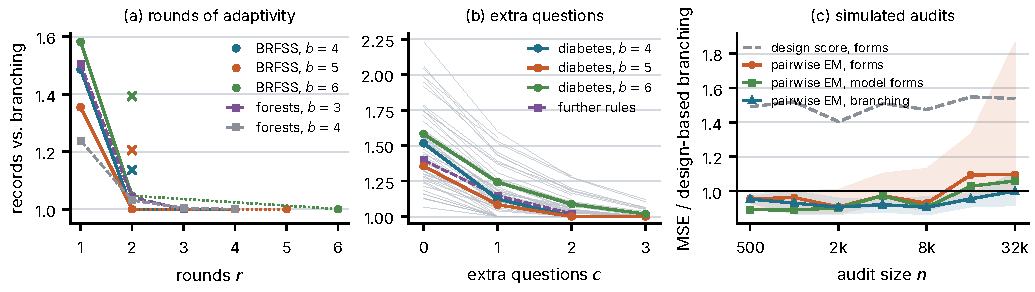
\includegraphics[width=\textwidth]{figures/v21_rounds.pdf}
\caption{What removes the price of pre-commitment on trained rules. Records needed relative to the branching interview with $b$ questions, without a model: (a) optimal $r$-round designs ($r=1$: fixed forms; $r=b$: branching) for BRFSS diabetes trees (median over runs; at $b=6$, $r=2$ includes upper bounds) and forest updates (median over tasks); crosses mark the heuristic of following the root question; (b) optimal forms with $c$ extra questions (thin lines: single rules; markers: medians over the rules computed at that size). (c) Simulated audits: mean squared error relative to the design-based mean under branching, for the design-based form score and for the pairwise EM estimate on three kinds of records (median over \nCurveTrees{} trees; bands: quartiles).}
\label{fig:rounds}
\end{figure*}

\paragraph{Q1: the price when the cap equals the depth.}
A depth-$b$ screening tree asks at most $b$ questions per person, so a validation study under the same burden must respect the cap. We train class-balanced CART trees on twelve yes/no items of the CDC Diabetes Health Indicators, derived from the Behavioral Risk Factor Surveillance System (BRFSS; 253,680 respondents, target diabetes or prediabetes) \citep{cdcdiabetes2017}, and on twelve binarized thyroid items \citep{quinlan1986thyroid}, and validate them on a disjoint random half or on respondents of the other sex. Branching administers the rule and takes a plain mean; the question is what forms lose against it. On thyroid, and whenever a tree uses at most $b$ items, one form asks everything the rule needs and nothing is lost. On BRFSS at caps four to six the best pre-committed design needs a median \nScreenBestLo--\nScreenBestHi{} times the respondents of branching (\nScreenRunLo--\nScreenRunHi{} over runs; Table~\ref{tab:screening}). \nRulesSentence

\emph{Ensembles.} For an old and a new random forest of twenty depth-$b$ trees (WDBC, Spambase, Ionosphere; $m\in\{6,9,12\}$ features) the contrast is the difference of predicted probabilities, which no single interview computes, so both classes face a design problem. At cap three the best forms need a median \nCapThreeMed{} times the records of the best branching design (range \nCapThreeMin--\nCapThreeMax), and an optimal two-round design at most \nTwoForestRatioMax{} times (Table~\ref{tab:capgrid}). Per question, the best forms cost \nCapQFixLo--\nCapQFixHi{} times complete records and the best branching designs \nCapQBrLo--\nCapQBrHi{} times (medians by cap): at the median capped forms roughly break even with complete records, and the cap pays clearly only if interviews branch. \nForestScaleSentence

\paragraph{Q2: what removes the price.}
\emph{Optimization.} Much of what a naive comparison credits to adaptivity is design optimization: uniform randomization over all forms of the rule's own items, with optimal tables, needs a median \nUitMedLo--\nUitMedHi{} times the records of branching by cap, and uniform matrix sampling over all twelve items \nUnifLo--\nUnifHi{} times. The numbers above are for oracle designs, tuned to the target law. Forms fitted on 20,000 complete source records need a median \nFitMed\% more and stay exactly unbiased; when such records exist and transport, imputation is a competitor (below). With no reference, the design is learned from a pilot charged to the audit (a quarter of $N=4{,}000$ records, cross-fitted): with cell masses smoothed by a pairwise fit it costs a median \nPilotAllLo--\nPilotAllHi\% more than the oracle of the same run, and without smoothing \nPilotEmpLo--\nPilotEmpHi\% more, the pilot being too small at $b=6$ (Tables~\ref{tab:screening} and~\ref{tab:pilotsmooth}).

\emph{Extra questions.} \nAugSentence

\emph{One more round.} Of the \nScreenGainN{} BRFSS diabetes trees with a gain, \nGainComputable{} are computed exactly by a two-round interview, \nGainExactNon{} more are within a factor \nScreenTwoMax{} of branching, and the remaining \nTwoBounded, at $b=6$, within \nTwoBoundMax{} (Figure~\ref{fig:rounds}a).

\paragraph{Q3: what a working model changes.}
A model buys efficiency with an assumption. \nCiSentence{} At the pairwise log-linear fit of each target law, forms need \nModelTwoLo--\nModelTwoHi{} times the records of the best branching design on the diabetes trees (\nModelAllLo--\nModelAllHi{} over all rules with at most ten items), where the design-based ratio at the same laws is \nModelDesignLo--\nModelDesignHi{} (Table~\ref{tab:model}); along the strongly coupled laws of Theorem~\ref{thm:structured}(c) the pairwise ratio rises from one to \nDepRatioLast{} at $b=3$ (Table~\ref{tab:dependence}).

\nMisspecSentence{} \nAuditParagraph

\paragraph{Further checks.}
An optimized design is tailored to one rule: scoring another tree on its records needs \nReuseMin{} to \nReuseMax{} times the records of branching, whereas one design shared by three known trees costs each a median \nJointPenMed\% more than its own optimum (Appendix~\ref{app:reuse}). Imputation from complete records of another population beats every capped design when it transports, and is biased in \nImpBadN{} of eight shift settings (Table~\ref{tab:shift}).
